% !TeX program = xelatex
% Compile with: xelatex -interaction=nonstopmode -halt-on-error -jobname=report_competition_review main.tex (three times)
\documentclass[UTF8,a4paper,zihao=-4,fontset=none]{ctexart}
% Template header begins 15 mm from the top; allow its full height above body text.
\usepackage[left=2.5cm,right=2.5cm,top=1.5cm,bottom=2.5cm,includehead,headheight=14mm,headsep=4mm,footskip=7.5mm]{geometry}
\usepackage{fontspec}
\setmainfont{Times New Roman}
\setsansfont{Arial}
\setmonofont{Consolas}[Scale=MatchLowercase]
\setCJKmainfont{SimSun}[AutoFakeBold=2]
\setCJKsansfont{SimHei}
\setCJKmonofont{SimSun}
\newCJKfontfamily\songti{SimSun}[AutoFakeBold=2]
\newCJKfontfamily\heiti{SimHei}[AutoFakeBold=2]
\usepackage{amsmath,amssymb,bm}
\usepackage{graphicx,booktabs,tabularx,array,multirow,longtable}
\usepackage{caption,float,placeins,needspace,setspace,enumitem}
\usepackage{fancyhdr}
\usepackage[numbers,sort&compress,square]{natbib}
\usepackage{xurl}
\urlstyle{same}
\usepackage[hidelinks,unicode,bookmarksnumbered]{hyperref}
\hypersetup{pdftitle={基于Zynq的相位运动放大与区域微振检测系统},pdfauthor={},pdfsubject={AMD FPGA赛道技术文档}}
\graphicspath{{figures/}}
\ctexset{
  section={name={第,部分},number=\chinese{section},format=\zihao{4}\heiti,beforeskip=18pt,afterskip=9pt},
  subsection={number=\arabic{section}.\arabic{subsection},format=\zihao{-4}\heiti,beforeskip=12pt,afterskip=6pt},
  subsubsection={number=\arabic{section}.\arabic{subsection}.\arabic{subsubsection},format=\zihao{-4}\songti,beforeskip=9pt,afterskip=4pt},
  paragraph={format=\zihao{-4}\songti,runin=false,beforeskip=6pt,afterskip=3pt}
}
\setcounter{secnumdepth}{3}
\setcounter{tocdepth}{2}
\setlength{\parindent}{2em}
\setlength{\parskip}{0pt}
\setstretch{1.5}
\clubpenalty=10000
\widowpenalty=10000
\setlength{\emergencystretch}{2em}
\newcolumntype{Y}{>{\raggedright\arraybackslash}X}
\renewcommand{\arraystretch}{1.25}
\setlength{\tabcolsep}{5pt}
\renewcommand{\small}{\fontsize{10.5pt}{13pt}\selectfont}
\renewcommand{\bibfont}{\zihao{5}\songti}
\captionsetup{font={small},labelfont=normalfont,labelsep=quad,justification=centering,singlelinecheck=false,skip=6pt}
\captionsetup[table]{position=top}
\numberwithin{figure}{section}
\numberwithin{table}{section}
\renewcommand{\thefigure}{\arabic{section}-\arabic{figure}}
\renewcommand{\thetable}{\arabic{section}-\arabic{table}}
\renewcommand{\theequation}{\arabic{equation}}
\newcommand{\reportfig}[4]{%
  \begin{figure}[!htbp]\centering
  \includegraphics[width=#2\linewidth]{#1}
  \caption{#3}\label{#4}
  \end{figure}}
\newcommand{\tabnote}[1]{\par\smallskip{\small\noindent #1\par}}
\setlist{nosep,leftmargin=2em}
\renewcommand{\topfraction}{.92}
\renewcommand{\bottomfraction}{.85}
\renewcommand{\textfraction}{.08}
\renewcommand{\floatpagefraction}{.75}
\setcounter{topnumber}{3}
\setcounter{bottomnumber}{2}
\pagestyle{fancy}
\fancyhf{}
\newcommand{\templateheader}{
\includegraphics[width=6.5158cm,height=1.1924cm]{template-header-logo.png}}
\fancyhead[C]{\templateheader}
\fancyfoot[C]{\fontsize{9pt}{11pt}\selectfont\thepage}
\renewcommand{\headrulewidth}{0.75pt}
\fancypagestyle{plain}{%
  \fancyhf{}%
  \fancyhead[C]{\templateheader}%
  \fancyfoot[C]{\fontsize{9pt}{11pt}\selectfont\thepage}%
  \renewcommand{\headrulewidth}{0.75pt}}
\begin{document}
\pagenumbering{Roman}
\thispagestyle{plain}
\begin{center}
{\zihao{3}\heiti\bfseries 基于Zynq的相位运动放大\par 与区域微振检测系统\par}
\vspace{.6em}
{\zihao{-4}\songti AMD FPGA赛道技术文档\par}
\end{center}
\noindent{\small 项目源码（GitHub）：\par
\noindent\url{https://github.com/cuijiaxin269-svg/FPGA_Visual_amplifier}\par}
\begin{center}{\zihao{4}\heiti 摘\quad 要}\end{center}
\addcontentsline{toc}{section}{摘要}

针对普通视频中微小振动难以辨识、运动位置与频率信息难以对应的问题，本作品设计了基于AMD Zynq-7000的相位运动放大与区域微振检测系统。系统面向振动与信号处理教学、机械结构低频振动观察，在同一板端终端上集成运动可视化、区域位移分析和交互控制。

系统采用OV9281采集$1280\times800$图像，由可编程逻辑完成多尺度分解、局部相位处理、时间滤波和图像重建；独立测量支路从原始采集帧的固定$256\times256$区域估计位移，经256点滑动窗口和直接离散傅里叶变换生成129个单边频点。FPGA以流水线、行缓存和专用运算模块承载密集计算，处理系统负责相机配置、帧调度、显示提交及串口屏交互，实现采集、计算、显示与控制的协同运行。

扬声器双频实板实验在5~Hz与10~Hz激励附近得到对应谱峰。v19补充记录完成三次断电冷启动、按键及触屏交互确认；两组黄金参考与HLS C模型比较中，已归档样例的最大绝对误差不超过1个RAW10码值。v18版本在固定配置下连续运行32分钟，平均处理速率为60.37969~frame/s，显示速率为30.00000~frame/s。Vivado~2025.2基线实现使用LUT~138026个、FF~206397个、BRAM~744.5个Tile和DSP~826个，BRAM利用率为98.61\%，WNS为$+0.177$~ns。资源分摊结果将主要片上存储开销定位到运动放大和ROI模块，为缓存复用与后续扩展提供了依据。

本作品通过整帧运动增强与原始ROI测量双支路设计，将运动形态和局部主频在同一终端对应呈现；通过缓存所有权管理、参数生效确认及启停排空机制，协调连续视频处理与用户操作，形成可独立运行的视觉微振观察与分析终端。

\vspace{.8em}
\noindent{\zihao{4}\heiti 关键字}\quad 相位运动放大；Zynq；区域位移估计；振动频谱；软硬件协同

\clearpage
\tableofcontents
\clearpage
\pagenumbering{arabic}
\section{作品概述}
\label{sec:overview}

\subsection{功能与特性}
本作品在AMD Zynq-7100平台上集成摄像头采集、微小运动可视化、区域位移分析和交互控制。摄像头对准被测物后，系统连续处理图像，通过HDMI输出原画、运动放大画面或带频谱面板的处理画面，使观察者能够同时查看运动位置、运动形态和局部主频。

系统包含两个处理支路：整帧相位运动放大支路增强细微运动的可见性，固定感兴趣区域（ROI）测量支路从原始采集帧估计位移并计算时间频谱。用户通过串口屏选择视图、设置相位增益$\alpha$与曝光、控制启动和停止；板端依据寄存器读回和任务完成状态反馈执行结果。$\alpha$为0--50的无量纲相位调制参数，用于调节运动增强强度。

外部硬件采用开发板、相机和显示设备；设计重点为相位算法的PL实现、双支路帧调度、视频叠加和串口交互，形成从图像输入到结果显示的完整处理链路。

\subsection{应用领域}
本作品面向振动、信号处理和嵌入式系统教学。观察扬声器膜片等低频振动物体时，普通视频中的细微运动不易辨识，频谱曲线也难以独立说明运动发生的位置。系统以原画作为观察基准，以放大画面呈现运动形态，以ROI位移谱显示局部频率组成，可用于讲解周期振动、双频叠加、图像相位处理及软硬件协同。5\,Hz与10\,Hz扬声器实验构成了具体的演示场景。

工程应用方向为支架、薄板、悬臂梁及隔振结构的低频振动辅助观察。视觉采集无需在被测物上安装接触式传感器，板端处理与显示便于在实验现场查看结果。开展不同支撑条件的对照时，应固定相机视角、曝光、激励和成像比例，并结合参考传感器建立频率与物理位移的对应关系。

\subsection{主要技术特点}
本作品以相位运动处理方法\cite{wadhwa2013}为基础，将多尺度分解、局部相位处理、时间滤波和图像重建部署到PL，并设置独立的原始ROI位移分析支路，同时输出运动增强图像与局部频谱。

连续视频包含大量重复像素运算，并要求采集、计算和显示接口协调工作。设计利用HLS流水线、行缓存及RTL视频逻辑构建专用数据通路，由PS执行相机配置、帧调度和交互控制。DDR保存图像帧及部分历史状态，BRAM保存局部缓存与算法工作区；运算资源、存储容量和任务依赖按照实际数据访问方式组织。

主要算法采用浮点计算。双支路共享原始采集帧，分别维护完成状态；参数更新、结果提交和缓存复用均受相应完成条件约束，以保持处理数据与界面状态一致。总体关系见图\ref{fig:system}。

\subsection{主要性能指标}
表\ref{tab:overview-metrics}汇总系统配置、v18实板吞吐与2025.2实现资源，测试条件见第三部分。

\begin{table}[htbp]
  \centering\small
  \caption{主要参数与结果概览}
  \label{tab:overview-metrics}
  \begin{tabularx}{\linewidth}{@{}p{0.24\linewidth}Xp{0.17\linewidth}@{}}
    \toprule
    项目 & 参数或结果 & 结果来源 \\
    \midrule
    输入/显示 & $1280\times800$/1080p30 & 配置 \\
    ROI/时间窗 & $256\times256$/256点 & 配置 \\
    LUT/BRAM/DSP & 49.76\%/98.61\%/40.89\% & 2025.2基线 \\
    处理/显示速率 & 60.38/30\,frame/s & v18实板 \\
    \bottomrule
  \end{tabularx}
\end{table}

\subsection{主要创新点}
本作品围绕算法部署与系统集成形成以下工程创新：

（1）组合整帧运动放大与原始ROI位移谱，使运动形态和局部主频在同一终端对应呈现。

（2）以PL专用计算、片上工作区及DDR帧缓存承载算法，由PS协调双支路输入帧的使用和释放。

（3）将寄存器读回、处理完成和启停排空纳入交互，以设备执行状态驱动参数反馈。

\subsection{设计流程}
设计流程包括需求分析、算法参考、软硬件划分、HLS/RTL/PS实现、模块测试、硬件实现和板级联调，如图\ref{fig:development}所示。根据测试结果定位问题，返回相应模块修正后重新检查功能与资源。大模型辅助源码检索、调试、数据整理、报告与视频脚本编制，作者校正场景和需求；通过日志、数值核对及PDF检查确认结果，形成协作总结与工程指南。

\reportfig{fig1-1-development.pdf}{1.0}{系统研发与验证流程}{fig:development}

\FloatBarrier
\section{系统组成及功能说明}
\label{sec:methods}

\subsection{整体介绍}
\subsubsection{系统总体架构}
系统由图像采集、运动可视化、区域位移分析、视频显示和人机交互五个部分组成。Zynq处理系统（PS）负责设备配置与任务调度，可编程逻辑（PL）负责图像计算、视频接收及显示输出。图\ref{fig:system}给出了各模块的数据连接和控制关系。

\reportfig{fig2-1-system.pdf}{1.0}{系统总体架构与数据通路。实线表示图像或数值数据，虚线表示主要控制与状态连接；两条算法支路均读取原始采集帧。}{fig:system}

OV9281图像经CSI接收和像素整理后，由采集DMA写入DDR原始帧缓存。每幅完整原始帧供两个支路读取：全帧支路执行多尺度相位运动放大，生成增强图像；区域支路提取固定ROI，估计二维位移并计算时间频谱。显示模块根据所选视图读取原始帧或增强帧，叠加ROI框、频谱及运行状态，经HDMI输出。区域测量始终使用原始采集帧，使位移分析与运动增强显示分别对应原始运动和可视化结果。

PS通过控制寄存器设置帧地址和算法参数、发出启动请求，并根据采集、计算及显示的完成事件调度下一项任务。用户通过串口屏或实体按键操作系统，独立日志串口输出调试信息。计算模块产生图像和数值结果，PS程序汇总任务状态并向界面反馈执行结果。

\subsubsection{数据通路与软硬件分工}
以$1280\times800$、60帧每秒计算，视频输入规模约为每秒6144万个像素，处理过程还包含空间滤波、相位运算和图像重建。本设计将这些重复密集的运算组织为PL流水线，按数据访问方式配置行缓存、FIFO和运算单元；初始化、命令解析及异步事件处理由PS执行。Zynq在同一器件内集成处理器与可编程逻辑，为这种分工提供了硬件基础\cite{ug585}。表\ref{tab:partition}列出了各项任务的执行位置及数据接口。

\begin{table}[htbp]
\centering\small
\caption{主要任务的软硬件划分}\label{tab:partition}
\begin{tabularx}{\linewidth}{@{}p{2.6cm}p{1.3cm}X X@{}}
\toprule
任务 & 位置 & 输入与输出 & 划分依据 \\
\midrule
相机配置及采集控制 & PS & 配置请求至传感器状态反馈 & 以软件组织寄存器配置、启停和异常处理 \\
CSI接收及采集DMA & PL & RAW10数据至DDR完整帧 & 对连续输入进行像素整理和帧写入 \\
相位运动放大 & PL & 原始帧至处理帧 & 以流水线组织多尺度和相位运算 \\
ROI位移及时间频谱 & PL & 原始ROI至位移、谱幅 & 独立配置二维变换与窗口处理资源 \\
视频时序及叠加 & PL & 显示帧、频谱至HDMI & 在像素通路内生成显示内容 \\
命令、调度及状态确认 & PS & 用户请求至实际状态反馈 & 统一管理缓存所有权与生效条件 \\
\bottomrule
\end{tabularx}
\end{table}

系统采用分层存储组织：DDR保存完整图像及部分历史状态，AXI承担批量读写；FIFO、行缓存和BRAM工作区服务于局部算子。整体吞吐由算子处理速率、任务依赖、缓冲深度和DDR访问共同决定。FPGA在本设计中承担可定制计算通路及视频接口集成，视觉采集方式则支持对被测物进行非接触观察。

\subsection{硬件系统介绍}
\subsubsection{硬件整体介绍}
系统采用OS-ZYNQ7100开发板，主芯片为AMD Zynq-7100，BOM型号为\texttt{XC7Z100-2FFG900I}，Vivado目标器件为\texttt{xc7z100ffg900-2}，使用板载DDR和QSPI存储。外设包括OV9281摄像头、HDMI显示器、串口屏及供电装置，扬声器作为实验中的振动对象。外围硬件复用现有平台，核心设计集中于HLS计算IP、RTL视频逻辑和PS控制程序。

\subsubsection{机械设计介绍}
实验采用支架固定摄像头并对准扬声器，开发板和串口屏放置在便于操作的位置，具体布置见第三部分整机照片。稳定的相机视角有助于减少支架晃动、桌面运动及遮挡对图像的干扰。观察距离、视角、照明和固定方式是运动对照测试的控制条件，应在采集过程中保持一致。

\subsubsection{电路各模块介绍}
摄像头接口包括配置通路和图像数据通路：PS执行传感器寄存器配置，PL接收MIPI/CSI数据。DDR保存原始帧、处理帧及部分历史状态，显示DMA与视频时序逻辑完成HDMI输出。串口屏通过UART1和EMIO通信，UART0输出日志，板上按键经GPIO参与视图控制，QSPI存储启动镜像。接口引脚由工程约束文件指定，UART接线遵循板卡I/O电平及共地要求。芯片BOM、供电说明与启动拨码照片归档于\path{board/hardware/}，引脚和串口电平约定见\path{board/wiring/README.md}；串口屏HMI/TFT工程与下载说明由\path{board/hmi/README.md}索引。

\subsection{软件系统介绍}
\subsubsection{软件整体介绍}
控制程序运行于Arm Cortex-A9裸机环境，负责相机驱动、HMI协议、帧调度和状态反馈。HLS算法经综合形成在PL中执行的专用计算模块，RTL实现采集、显示和信息叠加逻辑。控制程序通过寄存器接口调用计算模块，数据流、流水线及存储映射由HLS综合和Vivado实现流程确定\cite{ug1399,ug901,ug904}。

上电后，程序初始化平台、计时器、通信接口和诊断状态，进入待机轮询。收到合法启动请求后，程序结束旧显示缓存的读取、配置相机并启动采集，随后装载算法参数并准备位移窗口。运行期间，主循环响应采集、计算及显示完成事件，处理用户命令和错误状态。停止时，程序先等待采集DMA在帧边界停止，再等待在途计算及频谱任务完成，最后关闭相机输出并反馈停止状态。图\ref{fig:main-flow}给出了各阶段的转换条件。

\reportfig{fig2-3-main-flow.pdf}{1.0}{主程序运行流程。启动就绪和停止排空分别触发运行、停止反馈；停止后显示可保持末帧，故障进入错误清理分支。}{fig:main-flow}

\subsubsection{软件各模块介绍}
\paragraph{（1）图像采集与帧缓存管理}
采集链路接收$1280\times800$的RAW10图像，像素以16位容器存入帧缓存，有效值范围为0至1023。程序检查完整帧及校验状态后提交算法处理，通过原始帧三缓冲协调采集和读取。调度器分别记录采集写入、运动放大、ROI计算及显示读取的完成事件。两条计算支路均释放原始帧后，该缓存才重新交给采集DMA，保证ROI任务读取期间的数据保持完整。

\paragraph{（2）多尺度相位运动放大}
相位运动放大利用局部相位随运动变化的关系增强细小运动的可见性\cite{wadhwa2013}。本设计将原始帧分解为$1280\times800$、$640\times400$和$320\times200$三级空间带通信号，并保留$160\times100$的粗尺度残差。各尺度依次完成局部相位计算、时间带通滤波和相位调制，再通过逐级上采样与叠加重建图像，如图\ref{fig:phase}所示。

\reportfig{fig2-4-phase.pdf}{1.0}{多尺度相位运动放大流程。各尺度独立保存参考相位与历史滤波状态，下部展开单尺度的处理关系。}{fig:phase}

对某一尺度中的一个像素，记带通信号为$B_t$，两个方向的空间响应为$R_{x,t}$、$R_{y,t}$，记两方向空间响应的幅值为$r_t$，本实现的局部相位定义为
\begin{equation}
 r_t=\sqrt{R_{x,t}^{2}+R_{y,t}^{2}}+\varepsilon,
 \qquad \phi_t=\operatorname{atan2}(B_t,r_t),
 \label{eq:local-phase}
\end{equation}
其中$\varepsilon=10^{-6}$避免幅度项退化，$t$为帧序号。以首帧相位$\phi_0$为参考，得到$x_t=\phi_t-\phi_0$。二阶IIR采用转置直接Ⅱ型形式，其更新关系为
\begin{equation}
\begin{aligned}
 y_t&=b_0x_t+z_{1,t-1},\\
 z_{1,t}&=-a_1y_t+z_{2,t-1},\\
 z_{2,t}&=b_2x_t-a_2y_t.
\end{aligned}
\label{eq:iir}
\end{equation}
上述关系描述实时处理模式，带通系数$b_1=0$。首帧设置参考相位并将两个IIR状态置零，因此$x_0=y_0=0$，首帧带通信号直接通过。默认频带为3至12\,Hz；PS以历史基线采样率常数$f_s=60.379777$\,Hz计算IIR系数，运行时按配置装载。以$\alpha$调节带通相位后，子带重建为
\begin{equation}
 B'_t=B_t\cos(\alpha y_t)+r_t\sin(\alpha y_t).
 \label{eq:band-reconstruction}
\end{equation}
重建图像经过范围钳位与取整后写入处理帧缓存。$\alpha$用于调节带通相位，其数值与物理位移放大倍率采用不同定义；实际运动变化还受输入运动及滤波响应影响。

空间邻域运算通过行缓存复用相邻像素，算子之间通过流式FIFO连接，FIFO深度用于容纳不同尺度的启动和处理节奏差异。参考相位及两个IIR状态均采用单精度浮点，每像素共96位有效状态，四个像素的状态紧凑存为三个128位AXI字，内部计算流仍采用128位表示；打包和解包模块完成布局转换。

\paragraph{（3）区域位移估计与频谱分析}
ROI从原始采集帧中截取，左上角固定为$(512,272)$，尺寸为$256\times256$。ROI计算与全帧放大并行执行，以首个有效ROI建立参考。当前ROI经二维Hann窗和二维FFT处理后，与参考频域数据计算归一化互功率谱。本工程采用自定义硬件实现，相位相关的基本方法见文献\cite{opencvphase}。

\reportfig{fig2-5-roi-spectrum.pdf}{1.0}{ROI位移估计与时间频谱流程。二维FFT/IFFT用于空间位移估计，直接DFT用于连续位移样本的时间频谱。}{fig:roi}

记参考和当前ROI的频域数据为$F_0$、$F_t$，对应实现可写成
\begin{equation}
 C_t=\frac{F_0\overline{F_t}}{|F_0\overline{F_t}|+10^{-9}},
 \qquad c_t=\mathcal{F}^{-1}\{C_t\}.
 \label{eq:phase-correlation}
\end{equation}
算法在相关面$c_t$中搜索峰值，沿$x$、$y$方向分别采用三点抛物线插值，得到位移$\mathrm{d}x$、$\mathrm{d}y$，单位为像素（px）。按式\eqref{eq:phase-correlation}的互功率谱顺序，理想平移时输出为将当前ROI对齐到参考ROI所需的位移，其符号与当前图像相对参考图像的平移方向相反。低纹理、像素取值异常或无效帧对应参考失效状态，失效样本按无效测量处理。

连续有效位移进入256点滑动窗口。时间频谱模块对每个方向去均值、去线性趋势并施加Hann窗，以直接DFT计算129个单边频点。记预处理样本为$\widetilde d[n]$，则
\begin{equation}
 D[k]=\sum_{n=0}^{255}\widetilde d[n]\exp\left(-\mathrm{j}\frac{2\pi kn}{256}\right),
 \quad f_k=\frac{kf_s}{256},\quad 0\leq k\leq128.
 \label{eq:temporal-dft}
\end{equation}
其中$f_s$为位移采样率。按历史实验中约60.38\,Hz的采样率计算，窗口时长$256/f_s$约4.24\,s，频点间隔$f_s/256$约0.236\,Hz。模块以约5\,Hz发布频谱，每次输出使用最近256个连续有效位移样本，相邻输出共享重叠样本。帧序号不连续时清空旧窗口，再从当前有效样本开始积累。频点间隔确定频率网格，频率估计偏差由第三部分的双频实验给出。

\begin{table}[htbp]
\centering\small
\caption{关键算法与显示参数}\label{tab:algorithm-parameters}
\begin{tabularx}{\linewidth}{@{}p{3.0cm}p{3.4cm}X@{}}
\toprule
参数 & 配置 & 设计含义 \\
\midrule
相位增益$\alpha$ & 0至50，默认12 & 调节带通相位的调制量 \\
时间带通 & 默认3至12\,Hz & 根据频带及参考采样率计算IIR系数 \\
ROI & $(512,272)$，$256\times256$ & 从原始采集帧截取的固定区域 \\
频谱窗口 & 256个连续位移样本 & 输出129个单边频点 \\
频谱发布 & 约5\,Hz & 控制频谱更新节奏，相邻输出窗口重叠 \\
HDMI输出 & $1920\times1080$，30\,Hz & 显示接口的分辨率与刷新时序 \\
\bottomrule
\end{tabularx}
\end{table}

\paragraph{（4）并行任务调度与结果提交}
调度程序向运动放大和ROI模块提交同一原始帧地址，分别维护两路在途任务和完成标记，并在两路均释放输入后回收缓存。通过状态检查的增强帧提交给显示模块，ROI位移结果则按帧序进入频谱窗口。参数变化或停止请求到达时，程序先处理在途任务，再确认新配置或结束排空，保证配置变更前后的输出对应正确参数。相机采集、处理帧提交及显示刷新分别计数，用于分析各环节的运行速率。

\paragraph{（5）视频显示与信息叠加}
系统提供原画、放大无面板和放大带频谱面板三种视图。ROI框标出位移分析区域，频谱面板显示两个方向的谱幅及运行信息。PL将图像、叠加内容与显示时序组合后输出。频谱数值结果独立保存，屏幕柱高按显示量程映射；图像位移谱幅采用像素单位。停止采集与计算后，显示可保留末帧，运行状态由控制程序反馈。

\paragraph{（6）人机交互与参数生效机制}
串口中断负责字节收发，主循环执行命令解析和业务操作。控制程序分别维护请求接收、配置排队、参数应用及状态反馈，使界面提示与设备执行阶段相对应。主要命令及生效条件见表\ref{tab:hmi-commands}。

\begin{table}[htbp]
\centering\small
\caption{交互命令及生效条件}\label{tab:hmi-commands}
\begin{tabularx}{\linewidth}{@{}p{2.2cm}p{2.2cm}X@{}}
\toprule
命令 & 参数范围 & 实际生效与反馈条件 \\
\midrule
\texttt{VIEW} & 0、1、2 & 选择三种视图；停止时切换视图仍保持停止状态 \\
\texttt{ALPHA} & 0至50 & 参数读回匹配且新参数处理帧完成后确认 \\
\texttt{EXPOSURE} & 1至898 & 空闲状态接收并排队，下次启动写入相机及读回；运行时返回忙状态 \\
\texttt{START} & 无 & 等待采集、处理及显示满足就绪条件 \\
\texttt{STOP} & 无 & 停止采集并排空相关任务，取消待执行重启后确认 \\
\bottomrule
\end{tabularx}
\end{table}

\reportfig{fig2-6-parameter-sequence.pdf}{1.0}{参数应用与状态确认时序。左图为运行中修改相位增益，右图为空闲时设置曝光并在下次启动应用；箭头和纵向排列表示操作先后关系。}{fig:parameters}

如图\ref{fig:parameters}所示，程序等待当前算法任务结束后写入$\alpha$，在寄存器读回匹配且新参数帧处理完成后反馈增益生效；曝光值在空闲时排队，下一次启动时写入相机并读回。\texttt{RUNNING}反馈要求显示已启动且至少完成两次显示；放大模式还要求至少完成一帧算法处理。协议采用设备状态反馈格式，消息中不设置请求序号。

\paragraph{（7）启动加载与工程复现}
启动链路由BootROM、FSBL、位流和应用组成。位流、XSA、平台初始化文件及ELF成套管理，使硬件地址、平台配置和应用寄存器布局保持对应。仓库按源码、IP、仿真、构建、板端记录及数据组织目录，提供主机测试、ARM编译、RTL比对、硬件构建和启动包生成入口。工程复现依次进行环境配置、构建、产物哈希核对及对应板卡的部署测试。

报告对应的2025.2硬件构建以归档导出IP为输入，HLS源码用于算法与接口追溯。11月3日补充的源码重生成已完成五个模块的C仿真、生产配置综合和IP导出，有限RTL覆盖范围见第三部分；新候选IP不替换本文资源表所对应的封存IP。源码到IP的重生成、等价回归，以及启动包静态检查、Flash烧写、冷启动和业务运行，分别对应不同的复现步骤。各版本的测试对象和完成结果在第三部分列明，具体入口见第\ref{sec:reproduction}节。

\FloatBarrier
\section{完成情况及性能参数}
\label{sec:results}

\subsection{整体介绍}
作品已搭建由OS-ZYNQ7100开发板、OV9281相机、HDMI显示器和串口屏组成的实验系统，如图\ref{fig:system-photo}所示。相机安装在可调支架上，对准扬声器膜片；开发板完成图像处理与控制，HDMI显示器呈现视频结果，串口屏提供参数设置和启停操作。实验仪器用于产生和观察激励信号。系统采用现成板卡和外围设备，设计重点为图像算法的FPGA实现及采集、处理、显示和控制的联调。

\reportfig{system-overview.png}{0.82}{系统实验布置实物照片，包含被测扬声器、相机、开发板、串口屏、显示器及实验仪器。}{fig:system-photo}

\subsection{工程成果}
\subsubsection{机械成果}
相机采用现成支架固定，可调整高度与观察方向，使扬声器膜片位于成像范围内。开发板和显示终端采用桌面布置，便于接线、调试与操作。相机支架与被测物保持相对稳定，以减少拍摄装置晃动引入的图像位移。

\subsubsection{电路成果}
硬件集成完成相机输入、HDMI输出、串口交互和供电连接，复用开发板上的处理器、DDR及QSPI存储。板内逻辑由HLS计算IP和RTL视频通路组成，PS驱动程序负责设备配置与任务调度。外围接口与片上模块共同构成从图像采集到显示输出的处理链路。

\subsubsection{软件成果}
串口屏主界面如图\ref{fig:hmi-interface}所示。左侧选择原画、放大画面及详细参数视图，右侧调节相位增益和相机曝光，下方显示设备状态并提供启动入口。数值框承载用户设定，状态栏呈现设备反馈。增益生效以寄存器读回和新参数帧处理完成为判据，曝光生效以启动时的相机配置读回为判据，具体测试结果见第\ref{sec:interaction}节。

\reportfig{hmi-interface.png}{0.85}{串口屏主操作界面，包含视图选择、相位增益、相机曝光和启停控制。}{fig:hmi-interface}

\subsection{特性成果}
\subsubsection{测试环境与版本说明}
本文代码版本为V19（\texttt{v19boot}），整理后的工程固定于提交\texttt{a9ab041021c2}；2021.2与2025.2表示AMD工具版本。实验以扬声器为被测对象，检测固定ROI内的运动，并展示整帧相位运动放大结果。本节按测试版本列出板级运行结果、启动结果及Vivado~2025.2构建结果，见表\ref{tab:evidence-versions}。各项测试的原始数据和日志可通过仓库证据索引查阅\cite{repo}。

\begin{table}[htbp]
\centering\small
\caption{测试版本、条件与结果对应关系}\label{tab:evidence-versions}
\begin{tabularx}{\linewidth}{@{}p{2.7cm}p{3.2cm}X@{}}
\toprule
测试版本或材料 & 主要条件 & 已完成内容 \\
\midrule
扬声器双频实验 & 5\,Hz与10\,Hz激励，256个连续位移样本 & 对照设定频率检查位移谱峰 \\
v18hmi板级实验 & 串口交互、32分钟固定参数运行 & 命令响应及处理/显示速率测量 \\
v19补充验收 & 2021.2产物，11月3日三次断电上电及现场交互 & 冷启动、程序读回、KEY0、触屏与STOP确认 \\
黄金参考/C模型 & 两种尺寸，四组相位增益，同输入与帧映射 & 逐像素误差比较；输出来自HLS C仿真 \\
2025.2基线构建 & 提交\texttt{a9ab041021c2}及配套导出IP & 主机回归、RTL比对、硬件实现、固件编译及启动包静态检查 \\
实验场景图片 & 整机布置、原画与放大输出、串口屏界面 & 展示实物组成、显示模式和操作入口 \\
\bottomrule
\end{tabularx}
\end{table}

作者已确认整机上板可用。本节按实际来源区分证据：双频实验提供频谱记录，v18hmi提供固定配置连续运行和交互数据，11月3日的v19/2021.2记录提供补充验收结果，Vivado~2025.2基线提供资源与内部时序报告。不同版本分别保留，不将v19实测转记为2025.2构建产物的测量结果。

\subsubsection{运动放大效果}
图\ref{fig:display-comparison}展示同一扬声器场景的原画与放大输出。原画模式呈现相机采集的灰度图像，放大模式呈现相位处理后的图像；两种模式均叠加红色ROI框，标示原始帧中用于位移估计的固定区域。

\begin{figure}[htbp]
\centering
\begin{minipage}[t]{0.485\linewidth}
\centering
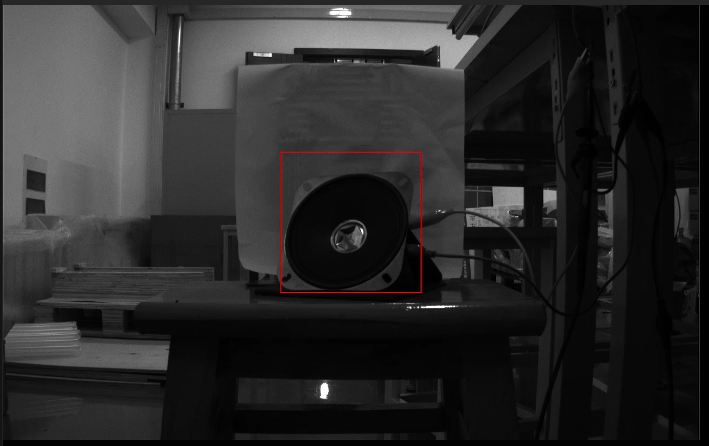
\includegraphics[width=\linewidth]{figures/display-original.png}
\par\small （a）原画面
\end{minipage}\hfill
\begin{minipage}[t]{0.485\linewidth}
\centering
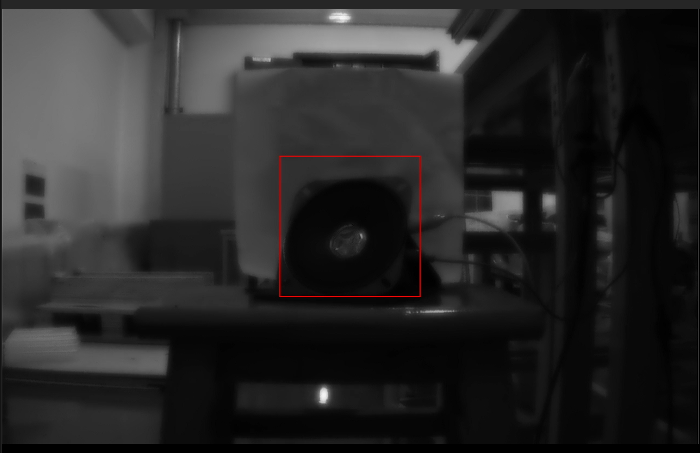
\includegraphics[width=\linewidth]{figures/display-amplified.png}
\par\small （b）放大输出画面
\end{minipage}
\caption{扬声器场景的原画与相位运动放大输出。两幅静态截图展示显示模式，红框标示固定ROI。}
\label{fig:display-comparison}
\end{figure}

系统将可视化与测量分开处理：运动放大支路生成显示图像，ROI支路直接从原始帧估计位移。本文位移及谱幅采用像素单位，$\alpha$表示相位调制强度；本节静态图比较不用于确定物理位移放大倍率。

\subsubsection{黄金参考与C模型数值比较}
补充数值比较使用同一输入、参数与帧映射，将独立黄金参考与HLS C模型输出逐像素对应。测试覆盖$64\times64$的128帧序列和$1280\times800$的8帧序列，均取$\alpha=0,12,30,50$。两组已归档样例的最大绝对误差均不超过1个RAW10码值。全尺寸结果见表\ref{tab:golden-comparison}，MAE与RMSE分别为全部像素的平均绝对误差和均方根误差。

\begin{table}[htbp]
\centering\small
\caption{全尺寸8帧黄金参考与HLS C模型输出比较}\label{tab:golden-comparison}
\begin{tabular}{@{}rrrr@{}}
\toprule
$\alpha$ & MAE & RMSE & 最大绝对误差 \\
\midrule
0 & 0 & 0 & 0 \\
12 & $1.2207\times10^{-7}$ & $3.4939\times10^{-4}$ & 1 \\
30 & $6.0168\times10^{-4}$ & $2.4529\times10^{-2}$ & 1 \\
50 & $8.0566\times10^{-6}$ & $2.8384\times10^{-3}$ & 1 \\
\bottomrule
\end{tabular}
\par\smallskip
\begin{minipage}{\linewidth}\small
注：误差单位为RAW10码值，像素范围0至1023。输出来源为主机HLS C仿真，非物理FPGA像素采集。
\end{minipage}
\end{table}

输入、参考、输出、逐帧误差与来源哈希由\path{board/results/v19_acceptance_20261103/}下的\path{golden_validation/}及\path{golden_validation_full/}索引，原始数组保存在完整验收附件。该比较验证所列样例的数值对应关系，不用于推导端到端延迟、实际位移放大倍率或板端逐像素误差。

\subsubsection{振动频率检测结果}
双频实验以5\,Hz和10\,Hz信号驱动扬声器，比较设定频率与图像位移谱峰的位置。固定ROI为$256\times256$，左上角坐标为$(512,272)$；时间谱由256个连续有效位移样本计算。

频谱读取程序重复读取结果缓冲区，并核对结果序号，仅接收两次读取一致的快照。9个候选快照中有3个满足该条件。图\ref{fig:spectrum-result}采用\texttt{spectrum\_00}：实测采样率为60.37956\,Hz，频点间隔约0.23586\,Hz，时间窗约4.24\,s；5\,Hz和10\,Hz附近的局部峰分别位于第21和42个频点，对应4.95301\,Hz和9.90602\,Hz，与输入频率对应。

\reportfig{fig3-5-spectrum.pdf}{1.0}{扬声器双频实板实验的ROI位移谱。纵轴为图像位移谱幅（px）；绘图保留原始频点，直流和奈奎斯特端点按单边谱定义修正，未作平滑或最大值归一化。}{fig:spectrum-result}

表\ref{tab:frequency-peaks}列出3个一致快照的插值峰值。六个峰值相对设定频率的绝对偏差为0.00231至0.02418\,Hz，说明该工况下能够分辨5\,Hz与10\,Hz输入。各快照取自同一连续采集过程，窗口可能重叠，表中偏差按快照列示，不作为独立重复测量的精度统计。图中约15、20、25、30\,Hz附近的附加分量保留在完整频谱中。

\begin{table}[htbp]
\centering\small
\caption{一致性通过快照中的频率峰值}\label{tab:frequency-peaks}
\begin{tabular}{@{}lrrr@{}}
\toprule
快照 & 目标频率/Hz & 插值峰值/Hz & 绝对偏差/Hz \\
\midrule
\texttt{spectrum\_00} & 5 & 5.01217 & 0.01217 \\
\texttt{spectrum\_00} & 10 & 10.00324 & 0.00324 \\
\texttt{spectrum\_05} & 5 & 5.02418 & 0.02418 \\
\texttt{spectrum\_05} & 10 & 10.00623 & 0.00623 \\
\texttt{spectrum\_06} & 5 & 5.00818 & 0.00818 \\
\texttt{spectrum\_06} & 10 & 9.99769 & 0.00231 \\
\bottomrule
\end{tabular}
\end{table}

\subsubsection{交互功能与边界测试}
\label{sec:interaction}
v18hmi交互实验通过真实UART链路测试\texttt{VIEW}、\texttt{ALPHA}、\texttt{EXPOSURE}、\texttt{START}和\texttt{STOP}五类命令。自动测试持续602631\,ms，共完成30轮交互；现场观察另记录了部分按键与屏幕操作。表\ref{tab:interaction-results}分别列出命令行为和验证方式。

\begin{table}[htbp]
\centering\small
\caption{v18hmi交互测试结果}\label{tab:interaction-results}
\begin{tabularx}{\linewidth}{@{}p{2.2cm}X p{3.1cm}@{}}
\toprule
动作 & 已记录行为 & 验证方式 \\
\midrule
VIEW切换 & 三视图与反馈状态对应；停止时切换不隐含启动 & 串口记录及部分现场确认 \\
ALPHA设置 & 范围与非法输入受控；新帧完成并读回匹配后确认 & 串口测试、增益操作反馈 \\
EXPOSURE设置 & 空闲时排队，下次启动应用；运行中返回BUSY & 串口测试及现场流程确认 \\
START / STOP & 就绪后报运行，排空后报停止；取消待执行重启 & 串口链路与状态读回 \\
按键与屏幕 & 视图同步，键盘编辑期间保护未提交内容 & 对应操作的现场观察记录 \\
\bottomrule
\end{tabularx}
\end{table}

曝光设置采用排队应用机制：空闲时保存新设定，启动采集前写入相机并核对读回值；运行中收到曝光修改请求时返回\texttt{BUSY}。停止后显示器可保持末帧，参数是否生效由设备反馈确认。

11月3日的v19补充记录保存了触屏切换至放大加频谱视图、KEY0两次切换及STOP操作。KEY0按下、受理和完成计数均为2；作者确认HDMI视图切换后恢复，STOP后屏幕显示停止且画面保持。三次真实断电上电均进入默认STOPPED状态，QSPI启动状态和运行程序读回相符。该补充记录按BOOT、位流、ELF和板内应用代码SHA256关联，入口为\path{board/results/v19_acceptance_20261103/README.md}。

\subsubsection{连续运行与处理速率}
v18hmi在VIEW~2、$\alpha=50$、曝光参数320的固定条件下连续运行32分钟。193个遥测采样点形成192个相邻区间，间隔约10\,s；处理帧计数增加115929，显示完成计数增加57600。按计数增量除以1920\,s计算，平均处理速率为60.37969\,frame/s，显示速率为30.00000\,frame/s。图\ref{fig:runtime-result}给出各区间结果，全程采集、算法及序列不连续等错误计数均为0。

\reportfig{fig3-6-runtime.pdf}{1.0}{v18hmi连续32分钟运行的区间处理与显示速率。阶梯线由计数差和时间差计算，虚线为时间加权平均；两面板纵轴跨度均为2\,frame/s。}{fig:runtime-result}

该结果表明，在上述输入和参数下，系统能够持续完成图像处理与30\,frame/s显示。曲线中的区间速率用于描述约10\,s尺度上的吞吐变化，上述计数不用于换算单帧端到端延迟。

v19补充记录的首尾计数跨度为2418.1\,s，处理计数增加146004，平均约60.3796\,frame/s；显示完成计数速率为30.0\,Hz，频谱发布约4.9857次/秒。该跨度包含234.1\,s的未观测间隙，期间存在调参和两次JTAG采集中断；累计有效观测为2184\,s。因此这些数据仅作为该版本板内计数端点速率，不替代v18固定配置32分钟连续运行结果，也不记为连续60分钟验收通过。

\subsubsection{FPGA资源利用率与实现约束分析}
\paragraph{实现后资源总量}
资源统计针对目标器件\texttt{xc7z100ffg900-2}上的完整设计\texttt{capture\_wrapper}，以Vivado~2025.2布局布线后的Physopt postRoute报告为准。图\ref{fig:utilization-result}直观展示各类资源的利用率，表\ref{tab:resource-total}给出精确数量。综合与实现报告为分析器件内映射和时序的依据\cite{ug901,ug904}。

\reportfig{utilization.png}{0.78}{FPGA资源利用率界面概览，百分比为取整显示；2025.2基线的精确数量与统计口径见表\ref{tab:resource-total}。}{fig:utilization-result}

\begin{table}[htbp]
\centering\small
\caption{2025.2完整设计的实现后资源占用}\label{tab:resource-total}
\begin{tabular}{@{}lrrr@{}}
\toprule
资源 & 已用数量 & 可用总量 & 利用率/\% \\
\midrule
LUT & 138026 & 277400 & 49.76 \\
LUT as Memory & 13029 & 108200 & 12.04 \\
FF & 206397 & 554800 & 37.20 \\
BRAM Tile & 744.5 & 755 & 98.61 \\
DSP & 826 & 2020 & 40.89 \\
Bonded IOB & 25 & 362 & 6.91 \\
BUFGCTRL & 4 & 32 & 12.50 \\
MMCME2\_ADV & 1 & 8 & 12.50 \\
\bottomrule
\end{tabular}
\par\smallskip
\begin{minipage}{\linewidth}\small
注：LUT as Memory包含在LUT总量内，不能重复相加；其中1424个用于分布式RAM、11605个用于移位寄存器。BRAM按36\,Kb Tile等效量统计。
\end{minipage}
\end{table}

\paragraph{片上存储与模块分摊}
BRAM使用744.5/755个Tile，容量余量为10.5个Tile，约1.39\%。其中708个RAMB36与73个RAMB18按$708+73/2$换算得到744.5个Tile。片上存储是利用率最高的主要资源，扩展缓存或增加ROI时应优先评估其容量和布局位置；DDR带宽则需依据访问量和运行测量单独分析。

表\ref{tab:resource-modules}按模块列出资源开销。运动放大模块使用391个BRAM Tile和557个DSP，ROI模块使用266个BRAM Tile和61个DSP，两者合计使用657个BRAM Tile，占已用BRAM的88.25\%，是存储优化的重点。表中四个模块合计使用673.5个BRAM Tile，占全设计BRAM用量的90.46\%，并包含全部826个DSP。完整设计还集成了离线时间滤波模块，其资源单独列入\texttt{f}实例。

\begin{table}[htbp]
\centering\small
\caption{主要模块的实现后资源分摊}\label{tab:resource-modules}
\begin{tabular}{@{}lrrrr@{}}
\toprule
模块及功能 & LUT & FF & BRAM Tile & DSP \\
\midrule
\texttt{motion}：运动放大 & 77542 & 117613 & 391 & 557 \\
\texttt{roi}：位移估计 & 8582 & 12084 & 266 & 61 \\
\texttt{spec\_fft}：时间频谱 & 4820 & 6853 & 6.5 & 12 \\
\texttt{f}：离线时间滤波 & 21461 & 31771 & 10 & 196 \\
\bottomrule
\end{tabular}
\par\smallskip
\begin{minipage}{\linewidth}\small
注：取同层实例统计，已包含各自子模块；不与下级资源再次累计。跨层次LUT合并可能影响子级加总，整体占用以顶层报告为准。
\end{minipage}
\end{table}

\paragraph{布局时序与扩展代价}
LUT、FF和DSP利用率分别为49.76\%、37.20\%和40.89\%，Slice占用为58571/69350，即84.46\%。功能扩展需要同时考虑资源组合、布局位置和布线需求。现有约束覆盖的内部时序中，WNS为$+0.177$\,ns、WHS为$+0.010$\,ns，TNS与THS均为0，建立与保持时序检查通过。MIPI~HS和HDMI的板外接口裕量不在该内部时序结果的覆盖范围内。

上述结果表明，完整基线设计已在目标器件上完成布局布线，BRAM是后续扩展的主要容量约束。优化方向为缩短缓存生存期、复用片上工作区，并结合数值误差评估存储位宽；评价时同时记录资源变化、输出误差、处理速率和时序余量。

\subsubsection{仿真回归与启动验证}
工程采用主机回归、软件/RTL比对、硬件实现和启动检查组成的验证流程，结果见表\ref{tab:validation-results}。主机回归检查协议与调度逻辑，软件/RTL比对检查频谱显示输出，综合实现检查资源映射和内部时序，启动包检查确认硬件平台与固件的配套关系。

\begin{table}[htbp]
\centering\small
\caption{验证层次及已完成范围}\label{tab:validation-results}
\begin{tabularx}{\linewidth}{@{}p{3.1cm}X p{4.1cm}@{}}
\toprule
验证项目 & 测试结果 & 检查对象 \\
\midrule
主机回归 & 8项测试通过 & 协议解析与调度逻辑 \\
频谱UI软件/RTL & Vivado~2025.2比对通过 & 软件参考与RTL显示结果的一致性 \\
2025.2基线实现 & 71个IP及顶层综合、布局布线和产物导出通过 & 完整基线设计的资源和内部时序 \\
固件与启动包 & 应用、FSBL构建及BOOT三分区静态检查通过 & 平台配置、分区组成及应用载荷 \\
v19补充验收 & 三次冷启动、KEY0两次操作及STOP检查通过 & 程序读回、计数记录与现场确认 \\
黄金参考/C模型 & 两种尺寸、四组增益；最大绝对误差不超过1 & 已归档HLS C输出，非板端像素输出 \\
HLS重生成阶段 & 五个模块C仿真、生产综合、导出及声明接口核对完成 & 原版源码；RTL与系统实现范围见下文 \\
\bottomrule
\end{tabularx}
\end{table}

11月3日19:48的HLS结果快照以原版提交\texttt{a9ab041021c2}为输入，使用Vitis HLS~2025.2、器件\texttt{xc7z100ffg900-2}和6.666667\,ns目标周期。五个模块已完成C仿真、生产配置综合与IP导出，声明接口核对一致；接口一致不等同于内部功能或实现时序等价。

RTL联合仿真中，复制模块以10组独立仿真、21次调用覆盖12个案例及11组相邻关系；频谱模块完成311个事务；时间滤波模块完成有界分组11次调用，AXI深度为15360，不外推至生产地址范围。ROI模块通过两个参数拒绝分支，正常路径尚未完成；运动放大模块已完成全尺寸C测试，完整帧RTL运行因资源限制中止。新候选IP的系统集成实现仍在进行，未纳入本文已通过的整机资源和时序结论。

各项测试保留输入、输出和结果记录，并将源码、硬件平台、位流、固件及启动包按版本关联归档。上述HLS阶段结论固定于所注明快照，完整验证及后续实现结果在完成后单独整理。

\subsubsection{资源优化设计与工程改进}
\paragraph{计算与存储的设计取舍}
表\ref{tab:design-tradeoffs}列出计算与存储的组织方法及其代价。设计以局部数据复用、紧凑状态布局和独立任务调度支撑连续视频处理，同时保留浮点算法的数值形式。

\begin{table}[htbp]
\centering\small
\caption{面向FPGA的计算与存储设计取舍}\label{tab:design-tradeoffs}
\begin{tabularx}{\linewidth}{@{}p{2.5cm}X X@{}}
\toprule
设计选择 & 具体组织与作用 & 资源及调度代价 \\
\midrule
行缓存与流水连接 & 空间邻域复用行缓存，算子间以FIFO传递数据 & 占用片上存储，FIFO深度需匹配各级启动和处理节奏 \\
相位状态紧凑存储 & 四组96位状态占三个128位AXI字，减少填充位 & 增加打包与解包逻辑，内部计算流保持原有接口形式 \\
共享原始帧与双支路 & 放大和ROI任务读取同一采集帧，分别维护完成状态 & 两路均释放输入后才能复用原始帧，需协调DDR访问与任务完成事件 \\
浮点运算与专用资源 & 相位、滤波及位移处理采用浮点计算并映射至PL & 浮点算子占用DSP与逻辑，位宽调整需同步评估数值误差 \\
\bottomrule
\end{tabularx}
\end{table}

在线模式的源码为每个像素保存参考相位与两个IIR状态，共$3\times32=96$位；四个像素共384位，打包为三个128位AXI字。相较每像素占用一个128位字的布局，该组织减少了状态填充位，并保持原有内部计算流接口。状态布局的作用是提高存储有效载荷比例，完整设计的资源占用见表\ref{tab:resource-total}。

\paragraph{已验证的工程修正}
串口接收、数值回包及重启状态管理中的问题和修正见表\ref{tab:engineering-revisions}。这些改进针对命令及时接收、数据访问约束及状态初始化，使控制流程与设备实际运行状态保持一致。

\begin{table}[htbp]
\centering\small
\caption{已记录的工程修正及验证范围}\label{tab:engineering-revisions}
\begin{tabularx}{\linewidth}{@{}p{3cm}X X@{}}
\toprule
原问题 & 实施处理 & 回归或实现结果 \\
\midrule
UART短包停留FIFO & RX触发阈值设为1，中断内排空FIFO & 对应主机及真实串口命令测试通过 \\
非对齐数值回包出错 & ARM构建保留禁止非对齐访问选项 & 对应版本重新测试通过 \\
空闲超时触发接收中断 & 禁用RX空闲超时，保留数据接收中断 & 接收处理由有效数据触发，减少空闲状态下的中断处理 \\
重启后遥测继承旧值 & 清零保留区并初始化中断、计时器状态 & v19交接及冷启动记录确认对应修正 \\
\bottomrule
\end{tabularx}
\end{table}

本节以设计结构和回归结果说明工程改进，以板级计数和实现报告分别给出吞吐及资源数据。后续量化优化收益时，应固定器件、工具、输入、参数和约束，在同一计时方法下比较输出误差、处理速率、BRAM/DSP占用及时序余量。

\subsubsection{工程复现与材料组织}
\label{sec:reproduction}
项目源码仓库为\url{https://github.com/cuijiaxin269-svg/FPGA_Visual_amplifier}，包含RTL、HLS与PS源码、构建脚本和验证记录。配套发布附件及使用方法见仓库README。完整演示视频与文件哈希见\path{media/video_manifest.json}；作者AI协作总结见\path{report/ai_logs/author_collaboration_summary_20261103.md}。11月3日配套资料的发布说明见\path{report/design_report/PUBLICATION_NOTE.md}，资料通过\texttt{materials-20261103}发布入口获取。

报告对应的代码基线为V19（\texttt{v19boot}）整理版，固定于提交\texttt{a9ab041021c2}；资源与时序来自该基线的Vivado~2025.2重新构建。完整提交号及文件哈希保存在配套清单中。已核对该提交的825项硬件输入、58项主机测试输入、6项频谱RTL验证输入和43项固件输入，均与构建记录的SHA256一致。重建原版工程时在独立目录检出该提交，并使用对应的位流、XSA、初始化文件和固件。该提交用于固定工程源码，11月3日新增的验收、黄金参考、屏端与硬件、视频及AI总结随当前资料版本提供；两者分别记录版本和哈希。

构建环境为Windows、AMD~2025.2工具、Python~3及包含标准头文件与库的C++工具链。硬件重建采用归档的导出IP；软件、仿真与硬件输出分别写入独立目录，保留各阶段结果。表\ref{tab:reproduction}列出执行顺序、入口和通过判据，命令参数及路径配置见仓库README和构建说明\cite{repo}。

\begin{table}[htbp]
\centering\small
\caption{工程复现顺序、入口与判据}\label{tab:reproduction}
\begin{tabularx}{\linewidth}{@{}p{2.0cm}p{6.5cm}X@{}}
\toprule
步骤 & 仓库内入口 & 通过判据 \\
\midrule
来源与文件核对 & \path{build/scripts/verify_package.py}\newline\path{report/evidence_index.md} & 文件清单、IP引用与目标版本一致 \\
主机及RTL验证 & \path{sim/scripts/run_host_tests.py}\newline\path{sim/scripts/run_spectrum_rtl.py} & 对应结果记录通过，保留输入和比较输出 \\
固件及硬件构建 & \path{build/scripts/build_firmware.py}\newline\path{build/scripts/build_hardware.ps1} & 检查结果记录、实现资源、约束内时序及导出产物 \\
启动包配套 & \path{build/scripts/build_boot.py} & XSA、位流、应用与FSBL成套，镜像检查和哈希一致 \\
实板功能验证 & \path{board/}及\path{report/evidence_index.md}中的对应版本记录 & 逐项确认采集、三视图、交互、停止排空及冷启动；保存实际日志 \\
\bottomrule
\end{tabularx}
\end{table}

重新构建或更换版本后的板级复测，应记录位流和ELF哈希、输入激励、ROI、曝光、相位增益、运行时长及判据。处理速率按处理帧计数增量计算，显示速率按显示完成计数计算；频谱检查应保存原始位移样本、窗口参数及数值结果。复测采集时，应按输入帧序号保存原画与处理输出，便于进一步分析位移与运动增强效果。

各阶段结果记录包含执行状态、输入文件哈希、输出位置和错误信息；通过版本清单将测试输入、构建产物与运行记录关联，便于复查设计结果和定位复现过程中出现的问题。

\FloatBarrier
\section{总结}
\label{sec:conclusion}

\subsection{可扩展之处}
资源优化优先针对运动放大和ROI模块开展缓存生存期分析，评估工作区复用、位宽调整和运算单元共享。在相同输入与约束下，同时比较数值误差、处理速率、BRAM/DSP占用和时序余量，确定各方案的收益与代价。

测量扩展按频率、纹理和振幅组织对照实验，引入参考传感器及成像比例标定，将像素位移转换为物理位移；在此基础上扩展可配置ROI与多区域分析。

下一阶段部署工作包括2025.2基线整机复测、冷启动验收、屏端源工程归档，以及HLS源码重生成与导出IP的等价比较，形成源码到板级运行的完整版本记录。

\subsection{心得体会}
\paragraph{软硬件协同与资源权衡}
视觉算法部署到板端后，计算、存储和任务调度相互影响。运动放大与ROI工作区是BRAM的主要开销来源，PS还要协调采集、计算和显示对帧缓存的使用。将模块资源分摊与帧完成记录结合分析，能够把资源开销对应到具体功能，并为缓存复用和任务调度调整提供依据。

\paragraph{大模型协作与证据核查}
在本次报告编制中，设计者确定应用定位、AMD评分重点、模板和素材；大模型辅助检索源码、整理数据、绘图及编写LaTeX。协作结果分别通过代码核对、原始数据检查、编译及PDF渲染确认。表\ref{tab:collaboration}列出三个具体案例，说明需求提出、修改执行与结果检查之间的对应关系。

\begin{table}[htbp]
  \centering\small
  \caption{报告编制中的协作案例与验证依据}
  \label{tab:collaboration}
  \begin{tabularx}{\linewidth}{@{}p{0.16\linewidth}Xp{0.22\linewidth}p{0.22\linewidth}@{}}
    \toprule
    实际问题 & 协作处理 & 检查依据 & 形成的方法 \\
    \midrule
    算法与版本标注 & 区分空间FFT、时间DFT、v18实板与2025.2实现 & 源码、数据及构建报告 & 每项指标记录算法、版本和条件 \\
    FPGA资源分析 & 汇总资源总量、模块分摊及BRAM余量 & 实现报告、模块资源表 & 从资源分布定位优化对象 \\
    图形与界面排版 & 横排流程图，更新串口屏UI并检查字号与分页 & 图形源文件、原始图像及PDF & 按最终插入尺寸检查可读性 \\
    \bottomrule
  \end{tabularx}
\end{table}

\paragraph{从工程经验到可复用技能包}
仓库将工程调试经验整理为三份指南\cite{repo}。《证据驱动的工程交接》从源码、产物哈希和测试目录建立版本对应关系；《串口控制与设备状态验证》依据原始字节、协议和状态表，逐层检查接收、解析、调度及完成事件；《启动镜像与冷启动验证》按镜像组成、传输、读回、自启动和外设业务划分检查步骤。

指南统一记录输入、操作步骤、完成判据和适用条件。文件核对、UART命令、实体触摸和外设运行分别保留对应结果，便于从异常现象追溯到具体环节。更换器件、工具链或协议时，先调整配置并核对适用条件，再执行相应步骤。

\Needspace{8\baselineskip}
\paragraph{版本一致性与复现经验}
源码、IP、初始化文件、位流和应用构成一套相互关联的交付物。复现文档同步记录工具版本、构建入口、输入参数、预期结果及原始日志路径；实板指标与实现报告分别注明版本和测试条件，使复现者能够沿同一入口检查功能、性能和产物对应关系。

\FloatBarrier
\section{参考文献}
\begingroup
\zihao{5}
\setstretch{1.25}
\renewcommand{\bibsection}{}
\begin{thebibliography}{9}
\bibitem{wadhwa2013}
WADHWA N, RUBINSTEIN M, DURAND F, et al. Phase-based video motion processing[J]. ACM Transactions on Graphics, 2013, 32(4): 80:1--80:10. DOI: \href{https://doi.org/10.1145/2461912.2461966}{10.1145/2461912.2461966}.
\bibitem{ug585}
AMD. Zynq 7000 SoC technical reference manual: UG585[EB/OL]. Version 1.15, (2026-02-06)[2026-11-01]. \url{https://docs.amd.com/r/en-US/ug585-zynq-7000-SoC-TRM}.
\bibitem{ug1399}
AMD. Vitis high-level synthesis user guide: UG1399[EB/OL]. Version 2025.2, (2026-01-22)[2026-11-01]. \url{https://docs.amd.com/r/2025.2-English/ug1399-vitis-hls}.
\bibitem{ug901}
AMD. Vivado design suite user guide: Synthesis (UG901)[EB/OL]. Version 2025.2, (2025-12-05)[2026-11-01]. \url{https://docs.amd.com/r/2025.2-English/ug901-vivado-synthesis}.
\bibitem{opencvphase}
OPENCV. Motion analysis and object tracking: phaseCorrelate[EB/OL]. Version 4.13.0[2026-11-01]. \url{https://docs.opencv.org/4.13.0/d7/df3/group__imgproc__motion.html}.
\bibitem{repo}
FPGA\_Visual\_amplifier：源码、构建说明与验证材料[CP/OL]. [2026-11-01]. \url{https://github.com/cuijiaxin269-svg/FPGA_Visual_amplifier}.
\end{thebibliography}
\endgroup

\end{document}
